
\NeedsTeXFormat{LaTeX2e}
\documentclass[letterpaper,10pt]{report}
\usepackage{natbib, graphicx, setspace, xcolor, lineno}
\usepackage{amssymb,amstext,textcomp,latexsym,amsmath}
\usepackage[framemethod=TikZ]{mdframed}
\bibliographystyle{apalike}


\mdfdefinestyle{MyFrame}{%
    linecolor=blue,
    outerlinewidth=1pt,
    roundcorner=10pt,
    innertopmargin=\baselineskip,
    innerbottommargin=\baselineskip,
    innerrightmargin=10pt,
    innerleftmargin=10pt,
    backgroundcolor=gray!50!white}

\begin{document}
\begin{center}

Supplementary material: Filtering Maps with GMT and Perl

Chuck Connor
February 6, 2014
\end{center}

\section*{Introduction}
Potential field map data are usually filtered with tools like Generic Mapping Tools and GeoSoft Montaj. Here we will work with Generic Mapping Tools (GMT) because it is free (!) and is easily used with Perl or python to ease calculations. We will work through an exercise in filtering magnetic map data. The data were collected by USF undergraduates in the San Rafael area in 2011, during their geophysics field camp. The San Rafael desert is in Utah (Figure~\ref{fig:survey}). This part of the San Rafael contains basaltic intrusions (dikes, sills, and volcanic conduits) hosted in sandstone. The basalts carry high magnetization (remanent and induced) and the sandstone is practically magnetically transparent. Let's go through step-by-step.


\begin{figure}
    \centering
    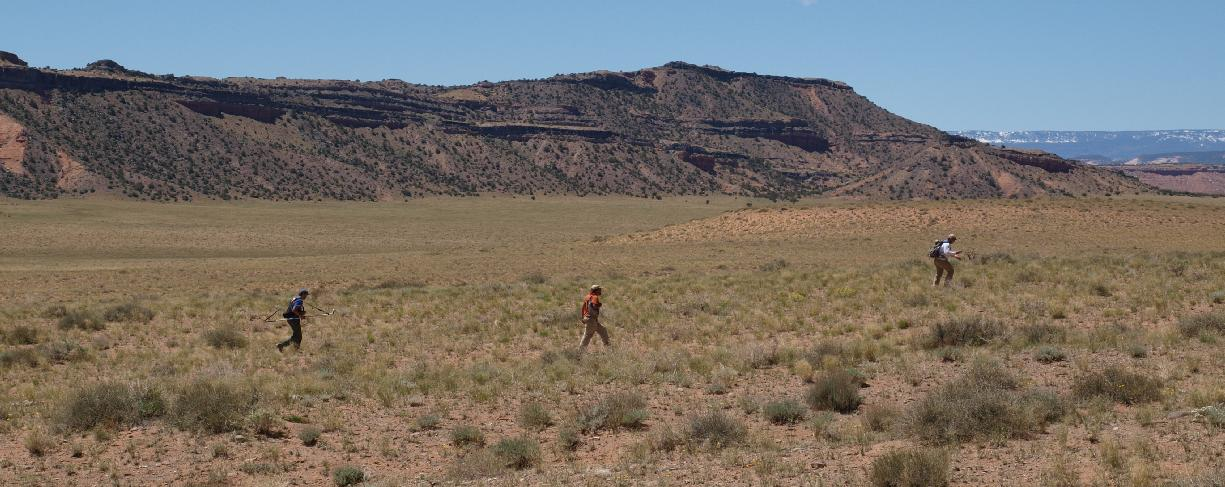
\includegraphics[scale=0.3]{./images/survey2.jpg}
    \caption{
Collecting magnetic data in the San Rafael area. Note that the area is characterized by relatively flat grass covered spaces devoid of outcrops. There are erosion resistent sills capping the sandstone cliffs in the background. Two volcano conduits are in the survey area (not shown on the photo).}
    \label{fig:survey}
\end{figure}


\section*{San Rafael Example}

The following example uses the data file {\it san\_raf\_mag.dat}. The data were collected with a total field magnetometer and a GPS. The format of the data file is: Easting (m), Northing (m), magnetic reading (nT), and elevation (m). That is:

\begin{verbatim}
480602	4264902 170.381000000001 1843
480602	4264902 170.387000000002 1843
480602	4264902 171.468000000001 1843
480603	4264902 173.821000000004 1843
.
.
.
\end{verbatim}
Note that the average regional field (IGRF) has already been removed from these data. The UTM coordinates are given in WGS84, zone 12. We want to visualize these map data and do some basic map filtering with the 2D FFT to enhance magnetic anomalies.

\subsection*{Step 1: Learn about the data}
Your first task is to learn about the range of values in the data file. Use the {\it gmt info} command to learn about the range of map values. That is, on the command line type:
\begin{verbatim}
gmt info san_raf_mag.dat
\end{verbatim}
Using the feedback from {\it gmt info} you can decide what map extent, scale, and contour interval are appropriate for the magnetic data. You may also want to plot a histogram of the magnetic readings, using {\it gmt pshistogram} or a similar tool. The histogram gives you a better sense of how the magnetic data are distributed by value (nT), also useful for selecting a contour interval.

\subsection*{Step 2: Plot the magnetic point locations}
You need to get a sense of how the magnetic readings are distributed in space. Use GMT to plot the data point locations, as well as other geologic data. In this case, other magnetic data are geological contacts, outlining two volcano conduits and the boundaries of a sill that outcrops in the E and SE portion of the map. The geologic data are located in separate files. For example, the file containing map location data of the sill contact {\it sill\_contact.xyz} has the format:
\begin{verbatim}
 480829.6802  4265068.3149  1825.3543 14:31:56  0.3022  0.4736  0.9304
 480829.7173  4265068.1549  1825.3651 14:31:57  0.3022  0.4736  0.9304
 480829.7544  4265067.9948  1825.3758 14:31:58  0.3022  0.4736  0.9304
 480829.7916  4265067.8348  1825.3866 14:31:59  0.3022  0.4736  0.9304
 480829.8287  4265067.6747  1825.3974 14:32:00  0.3064  0.4797  0.9430
 480829.4981  4265067.0312  1825.2029 14:32:01  0.3099  0.4884  1.0012
 480829.1676  4265066.3876  1825.0085 14:32:02  0.3099  0.4884  1.0012
.
.
.
\end{verbatim}
These data include the Easting, Northing, and elevation of the contact, measured at a particular time. The last three columns show the reported GPS accuracy, in uncertainty E-W, N-S, and vertical, which are probably over-estimates. The following script illustrates plotting the data on a map with Perl and GMT:
\begin{mdframed}[style=MyFrame]
\begin{verbatim}
$in = "san_raf_mag.dat";
$out = "san_raf_points_map.eps";

$plugL = "./geology/plug1.xyz";
$condL = "./geology/plug1_base.xyz";
$condS = "./geology/plug2_base.xyz";
$sill = "./geology/sill_contact.xyz";

$west = 479500;
$east = 480900;
$south = 4264100;
$north = 4266000;

system "gmt psxy  $in -R$west/$east/$south/$north -Jx1:12000
   -Sp -W0.5p,255 -Ba400f50:'':/a200f50:'':/WSne -V -K > $out";
system "gmt psxy  $condL -R -Jx -N -Sc.02i -W1p 
   -O -K -V >> $out";
system "gmt psxy  $condS -R -Jx -N -Sc.02i -W1p
   -O -K -V >> $out";
system "gmt psxy  $plugL -R -Jx -N -Sc.02i -W1p 
   -O -K -V >> $out";
system "gmt psxy  $sill -R -Jx -Sc.02i -W1p -O -V >> $out";

system "gmt ps2raster $out -A -P -Tg";
system "rm $out";
\end{verbatim}
\end{mdframed}
\vspace{2 mm}
The first thing to notice about this Perl script is that it specifies the names of input and output files as variables:
\begin{verbatim}
$in = "san_raf_mag.dat";
$out = "san_raf_points_map.eps";
\end{verbatim}
This is useful because you will not have to search the rest of the script to find places where the file names are called out if you decide to use a different file. There may be many lines of code where the file name appears! Note that the file names for data files containing geologic data are also specified. These data files are located in a directory call {\it geology}. It is extremely useful to create a directory for such files to keep your work organized. Similarly, variables are defined to specify the geographic boundaries of your map, here in UTM coordinates.

The next command in the script actually creates the map using these and additional specifications.
\begin{verbatim}
system "gmt psxy  $in -R$west/$east/$south/$north -Jx1:10000 -Sp -W0.5p,255
   -Ba200f50:'Easting (m)':/a100f50:'Northing (m)':/WSne -V -K >> $out";
\end{verbatim}
The GMT program {\it psxy} actually creates the map. The other arguments on the line specify how the map will look, what data will be used (\$in), and the name of the map file -- specified by \$out. Look for the specific meanings of -R, -J, -S -W, -B and -V, on the GMT man page for {\it psxy} by typing on the command line:
\begin{verbatim}
man gmt psxy
\end{verbatim}
Pay particular attention to the end of the line:
\begin{verbatim}
-K > $out";
\end{verbatim}
The -K option lets GMT know that additional information will be added to the output map file. The $>$ symbol redirects the output to the file \$out. Next, the additional geologic data are plotted on the map. Note the syntax in these lines:
\begin{verbatim}
-O -K >> $out";
\end{verbatim}
This syntax indicates that data will be Overlayed on the existing plot (-O) and more data will follow (-K). Notice $>>$ is used to indicate that the information is appended to (added to) the \$out map file. Notice in the last {\it gmt psxy} line, the -K switch is not used, because no more information will be added.

When this script is successfully run, your output should look like that shown in Figure~\ref{fig:points}.



\begin{figure}
    \centering
    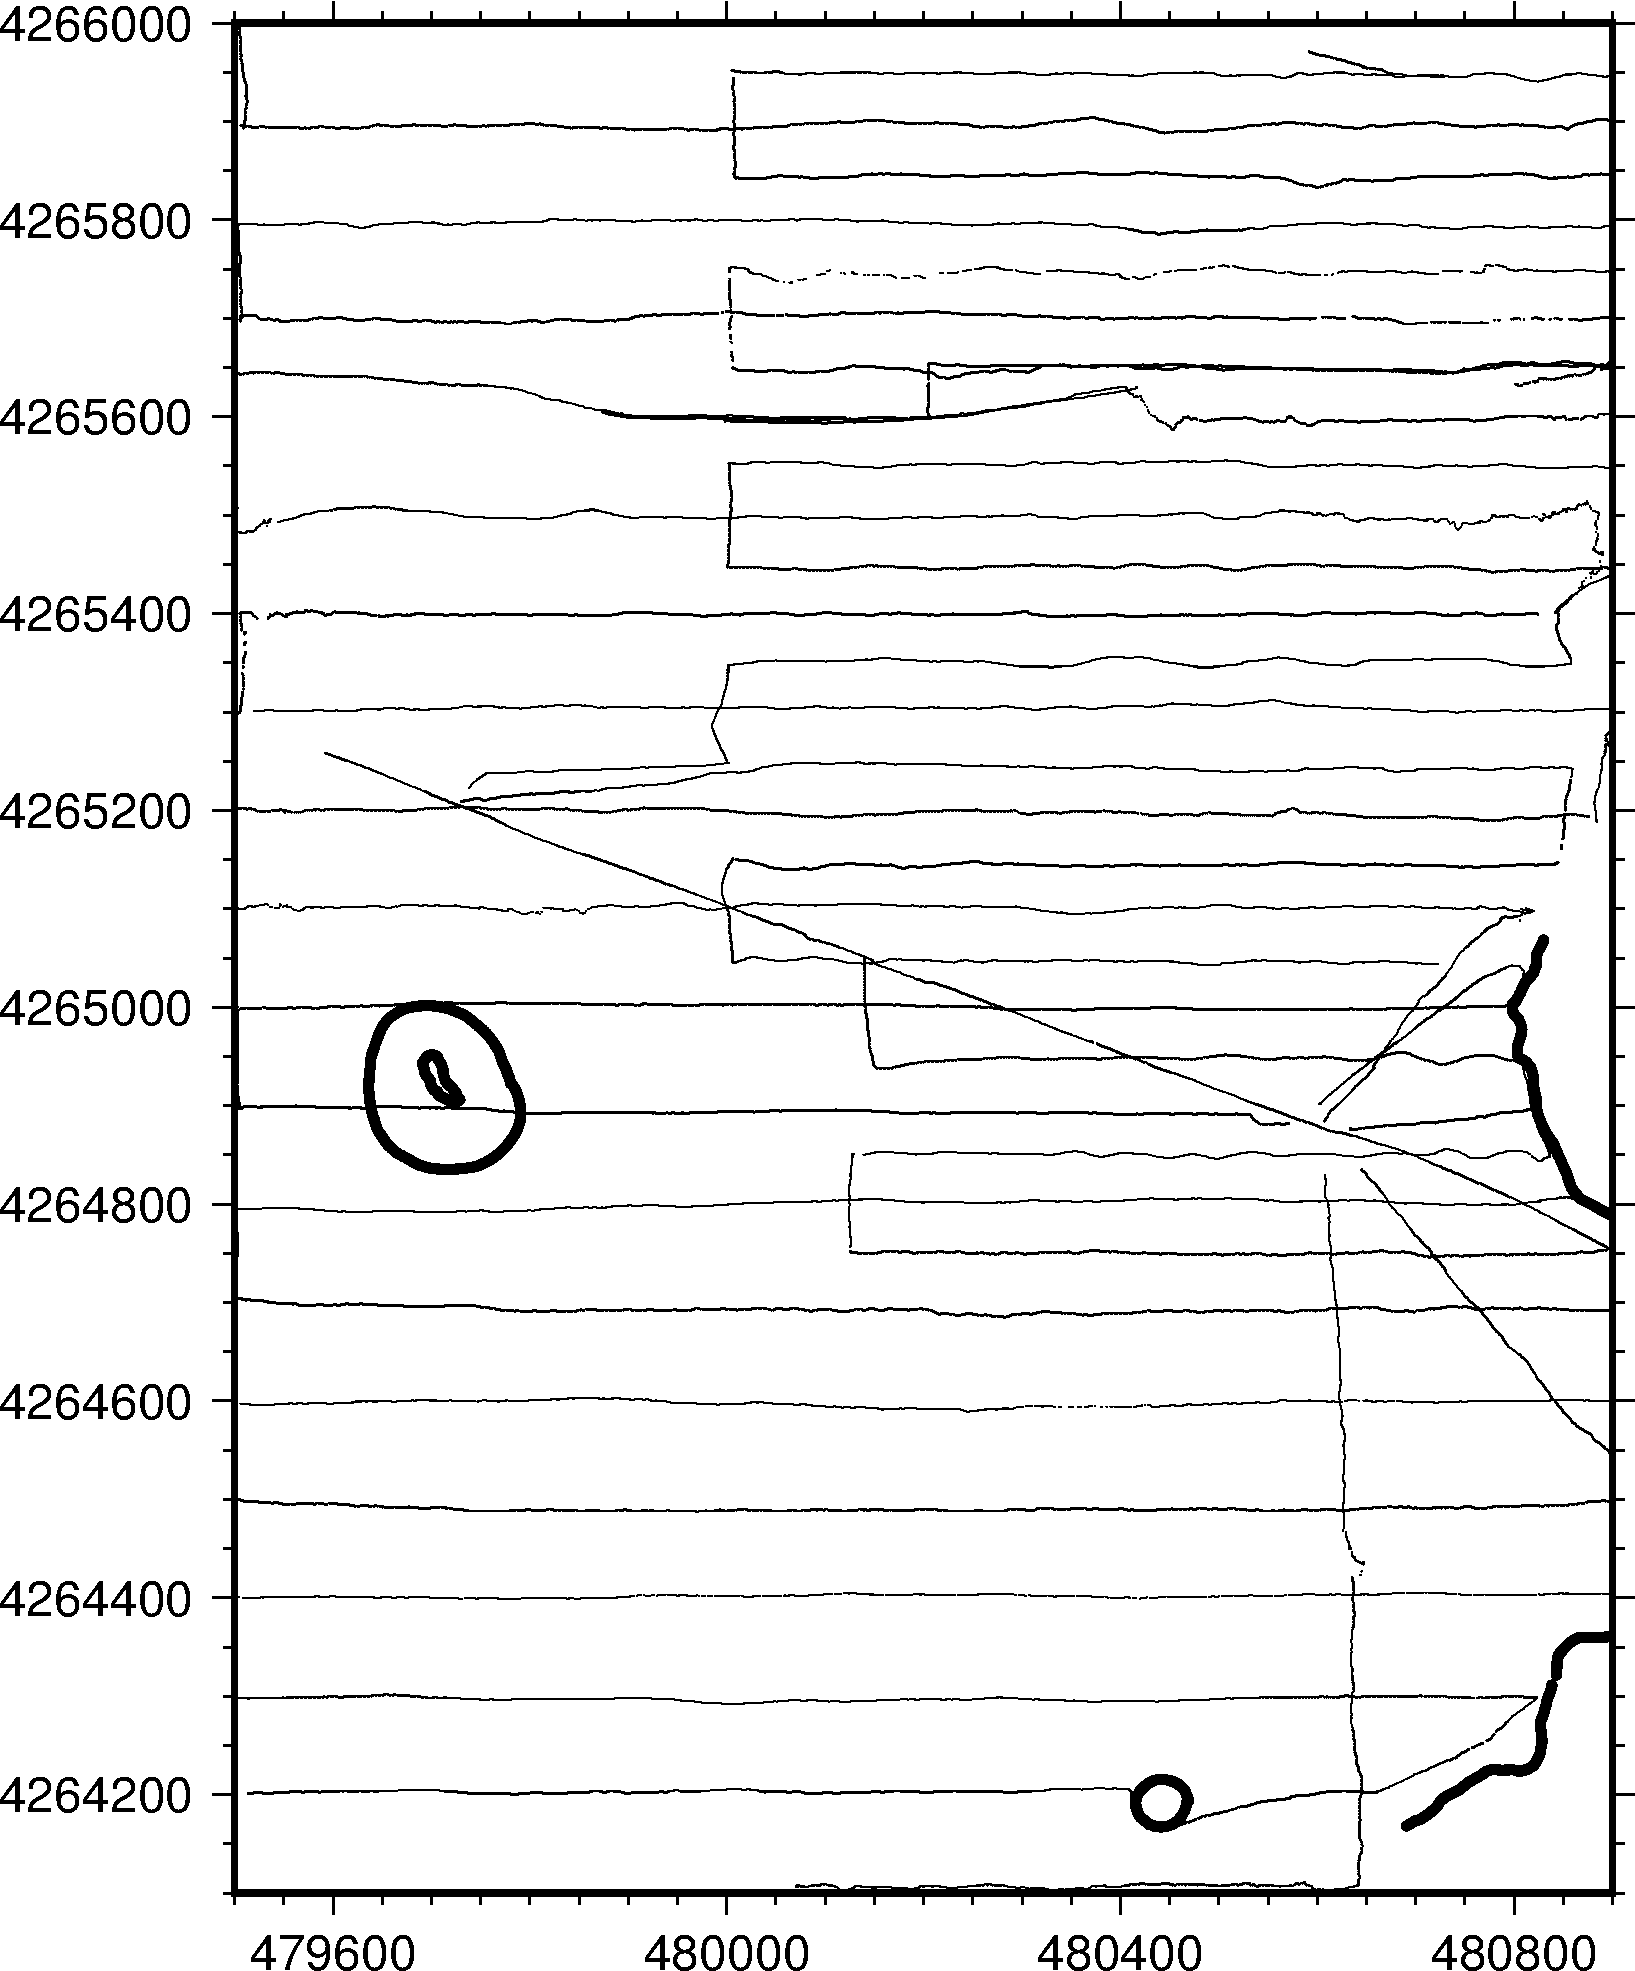
\includegraphics[scale=0.75]{./images/san_raf_points_map.png}
    \caption{
Output from running the the script in Step\,2 to plot magnetic data points and geologic contacts.}
    \label{fig:points}
\end{figure}


\subsection*{Step 3: Making the contour plot and image}
Visualizing the magnetic data involves contouring and making an image of the variation in the magnetic field across the survey area. The following script accomplishes this.
\begin{mdframed}[style=MyFrame]
\begin{verbatim}
$in = "san_raf_mag.dat";
$out = "san_raf_mag_map.eps";

$plugL = "./geology/plug1.xyz";
$condL = "./geology/plug1_base.xyz";
$condS = "./geology/plug2_base.xyz";
$sill = "./geology/sill_contact.xyz";

$west = 479500;
$east = 480900;
$south = 4264100;
$north = 4266000;

$color_file = "haxby";
$min_value = -200;
$max_value = 600;
$cint = 20;

# grdcontour
$anot_int = 100;
$contours = 50;

# psscale
$xpos = 12.5;
$ypos = 8.4;
$len = 8;
$width = .25;
$orient = "v";
$scale_anot_int = 50;

system "gmt surface $in -I5 -Gsurf.grd 
   -R$west/$east/$south/$north -V";
system "makecpt -C$color_file 
   -T$min_value/$max_value/$cint -V > map.cpt";
system "grdimage surf.grd -Jx1:12000 -Cmap.cpt 
    -Ba400f50:'':/a200f50:'':/WSne -K -V > $out";
system "grdcontour surf.grd -R -Jx -C$contours 
    -W0.25p,100 -O -K >> $out";
system "gmt psxy  $in -R -Jx -Sp -W0.5p,255 
    -O -K -V >> $out";
system "gmt psxy  $condL -R -Jx -N -Sc.02i -W1p 
    -O -K -V >> $out";
system "gmt psxy  $condS -R -Jx -N -Sc.02i -W1p 
    -O -K -V >> $out";
system "gmt psxy  $plugL -R -Jx -N -Sc.02i -W1p 
    -O -K -V >> $out";
system "gmt psxy  $sill -R -Jx -Sc.02i -W1p 
    -O -K -V >> $out";

system "psscale -D$xpos/$ypos/$len/$width$orient 
    -Cmap.cpt -B$scale_anot_int:'Magnetic Anomaly':/:nT: 
    -O -V >> $out";

system "ps2raster $out -A -P -Tg";
system "rm $out";
\end{verbatim}
\end{mdframed}
Most of this code is identical to the script used to plot the magnetic data points in Step\,2. Some additional variables are created to control the map. 
\begin{verbatim}
$color_file = "haxby";
$min_value = -200;
$max_value = 600;
$cint = 20;
\end{verbatim}
These variables control the colors used to create the image of variation in the magnetic field, and the range in magnitude of magnetic values represented by the colors. You can experiment by changing the range and the color table to see how the map changes. These lines
\begin{verbatim}
$anot_int = 100;
$contours = 50;
\end{verbatim}
control the contour interval and the interval at which contour lines are labeled (usually). These lines
\begin{verbatim}
$xpos = 12.5;
$ypos = 8.4;
$len = 8;
$width = .25;
$orient = "v";
$scale_anot_int = 50;
\end{verbatim}
control the position of the color bar. This line does the work of interpolating the data onto a grid:
\begin{verbatim}
system "gmt surface $in -I5 -Gsurf.grd 
   -R$west/$east/$south/$north -V";
\end{verbatim}
It specifies that the data in \$in will be interpolated onto a grid, that the grid spacing will be 5 map units (in this case meters), that the grid will have the map extent, -R, and the grid will be sorted in a new file called {\it surf.grd}. Then the image is made and contours drawn on the image:
\begin{verbatim}
system "makecpt -C$color_file 
   -T$min_value/$max_value/$cint -V > map.cpt";
system "grdimage surf.grd -Jx1:12000 -Cmap.cpt 
    -Ba400f50:'':/a200f50:'':/WSne -K -V > $out";
system "grdcontour surf.grd -R -Jx -C$contours 
    -W0.25p,100 -O -K >> $out";
\end{verbatim}
You can experiment, for example by changing the contour interval and the width of the contour lines. Also experiment by changing the grid spacing. Your output will look something like shown in Figure~\ref{fig:contour}. 


\begin{figure}
    \centering
    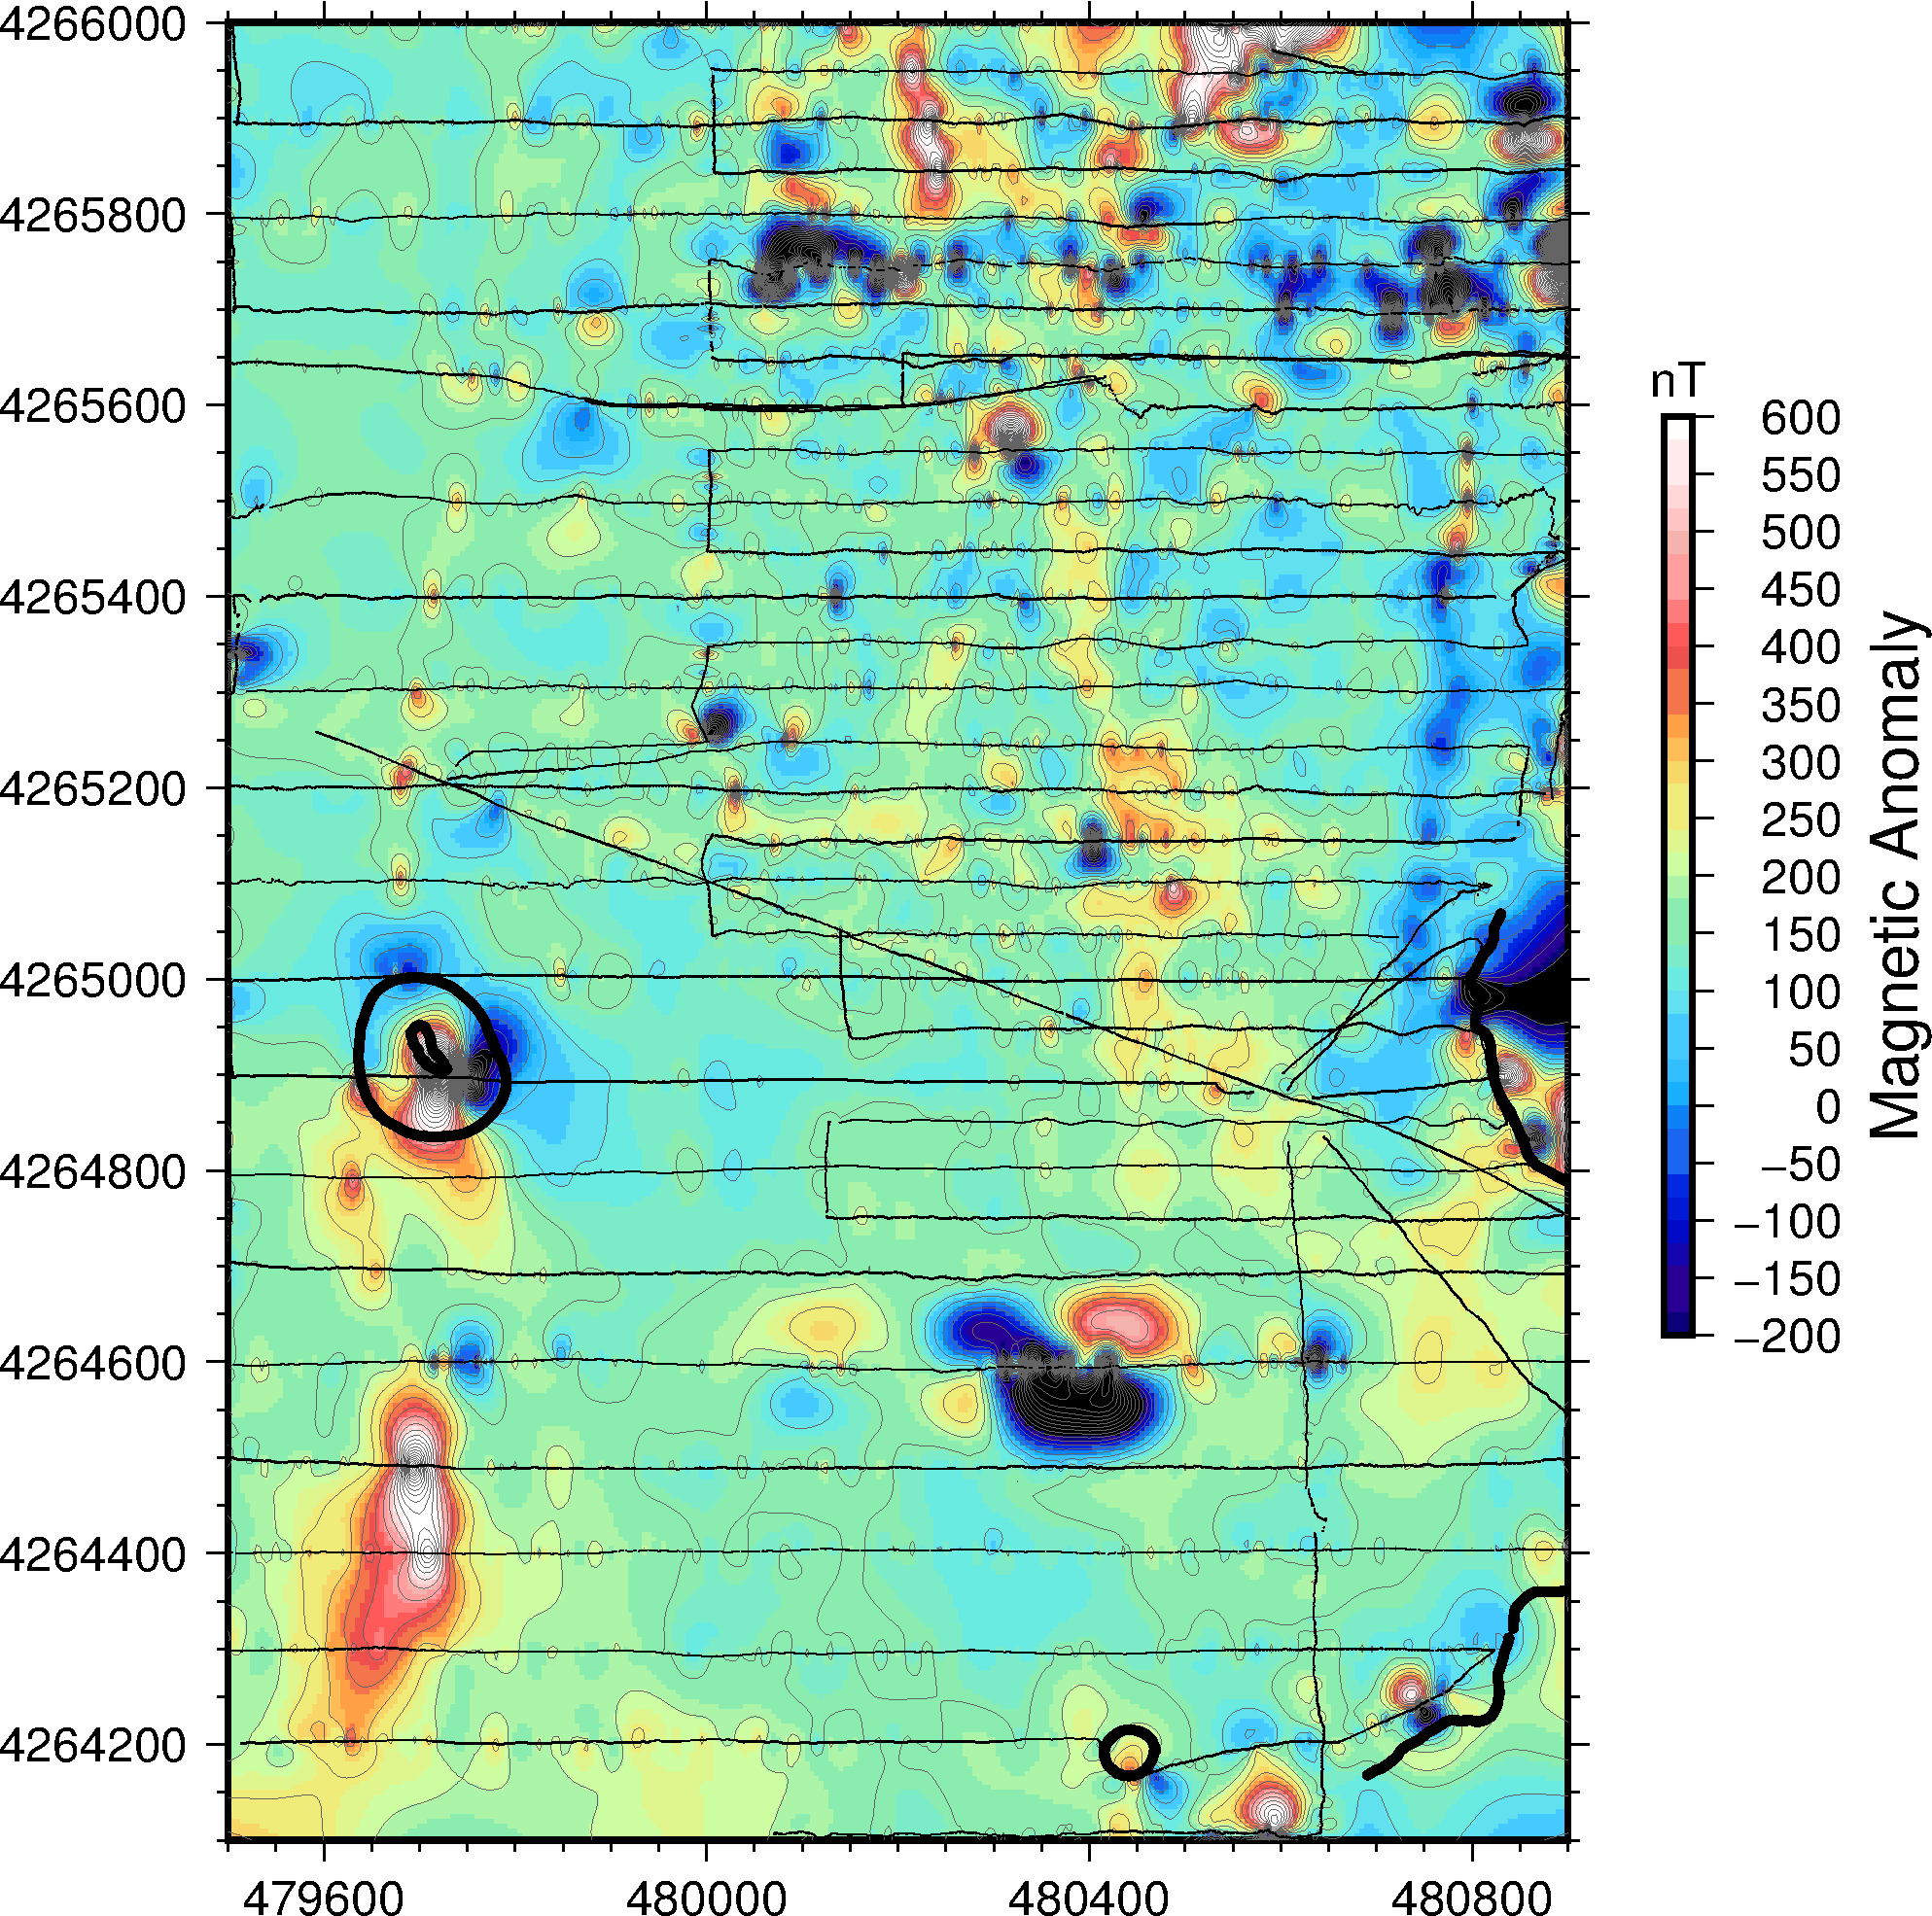
\includegraphics[scale=0.75]{./images/san_raf_mag_map.png}
    \caption{
Output from running the the script in Step\,3 to make the magnetic map and overlay geologic contacts.}
    \label{fig:contour}
\end{figure}


\subsection*{Step 4: Deleting bad data}
Things sometimes go wrong in the field and bad data are collected. For example, on the San Rafael survey, some data were collected by students who either wore too much metal, or were collecting data near someone who wore too much metal. Perl is an efficient tool for deleting bad sections from data sets. Inspection of Figure~\ref{fig:contour} shows some sections that have bad data. The following perl script filters the map data to remove one of these sections.\\
\vspace{3 mm} 

\begin{mdframed}[style=MyFrame]
\begin{verbatim}
open(MAG, $ARGV[0]) || die "Cannot open <$ARGV[0]> for
     input: [$@]";
@LINES = <MAG>;

$ct = 0;

foreach my $line (@LINES) {
  ($e, $n, $mag, $el ) = split " ", $line;
  if (($n > 4264550 && $n < 4264650) && 
            ($e>480260 && $e <480480)) {
  	$ct++;
  	print stderr "$e $n $mag $el\n";
     
  }
  else {
  	 print "$e $n $mag $el\n";
  }
}
print stderr "Removed $ct lines\n";
\end{verbatim}
\end{mdframed}
\vspace{3 mm}
Run this script to filter your data set to remove data in the area indicated by the conditional statement (if...). Replot your data points to make sure you deleted the right section. It turns out that all data collected along line 4265750N -- say within 25\,m of this Northing coordinate -- are also bad. Make sure you filter out these bad data as well. Re-grid and re-contour the make and make sure the map has improved! 

\subsection*{Step 5: upward continuation}
GMT really comes into its own as a powerful tool in geophysics when we start filtering maps. We are ready to use the FFT to filter the gridded magnetic map, using the GMT code {\it gmt grdfft}. Basically to do an upward continuation the following lines need to be modified and added to the script you created in Step\,3, now using the input data set that filtered out bad points, of course (see Step\,4). 
\begin{verbatim}
system "gmt surface $in -I5 -Gsurf.grd 
           -R$west/$east/$south/$north -V";
system "gmt grdfft surf.grd -Gfiltered.grd -C10 -V";
system "gmt makecpt -C$color_file -T$min_value/$max_value/$cint -V > map.cpt";
system "gmt grdimage filtered.grd -Jx1:12000 -Cmap.cpt -Ba400f50:'':/a200f50:'':/WSne 
             -K -V > $out";
system "gmt grdcontour filtered.grd -R -Jx -C$contours -W0.25p,100 -O -K >> $out";
\end{verbatim}
The key change in the use of {\it gmt grdfft} to upward continue the gridded data set. This produces a new grid file, here named {\it filtered.grd}. Then this new filtered grid is imaged and contoured. The -C argument is used to upward continue the map grid by 10 map units (10 meters in this case). Of course, upward continuation attenuates the signal, so you probably have to choose new values for your color scale and contour interval. 

\subsection*{Step 6: Reduction-to-pole}
Similar to upward continuation and other filtering processes, reduction-to-the-pole is straightforward using GMT. The {\it gmt grdredpol} program is used. In the following example the -C argument is used, which is the ``classic reduction to pole".
\begin{verbatim}
system "gmt surface $in -I5 -Gsurf.grd 
         -R$west/$east/$south/$north -V";
system "gmt grdfft surf.grd -Gfiltered.grd -C10 -V";
system "gmt grdredpol filtered.grd -Grtp.grd -C0/50 -V";
system "gmt makecpt -C$color_file -T$min_value/$max_value/$cint -V > map.cpt";

system "gmt grdimage rtp.grd -Jx1:9000 -Cmap.cpt 
       -Ba200f50:'Easting (m)':/a100f50:'Northing (m)':/WSne -K -V > $out";
system "gmt grdcontour rtp.grd -R -Jx -C$contours -W0.25p,100 -O -K >> $out";
\end{verbatim}
Figure~\ref{fig:rtp} shows the resulting map. Experiment with different values of inclination and declination and not the affect on the appearance of the map!

\begin{figure}
    \centering
    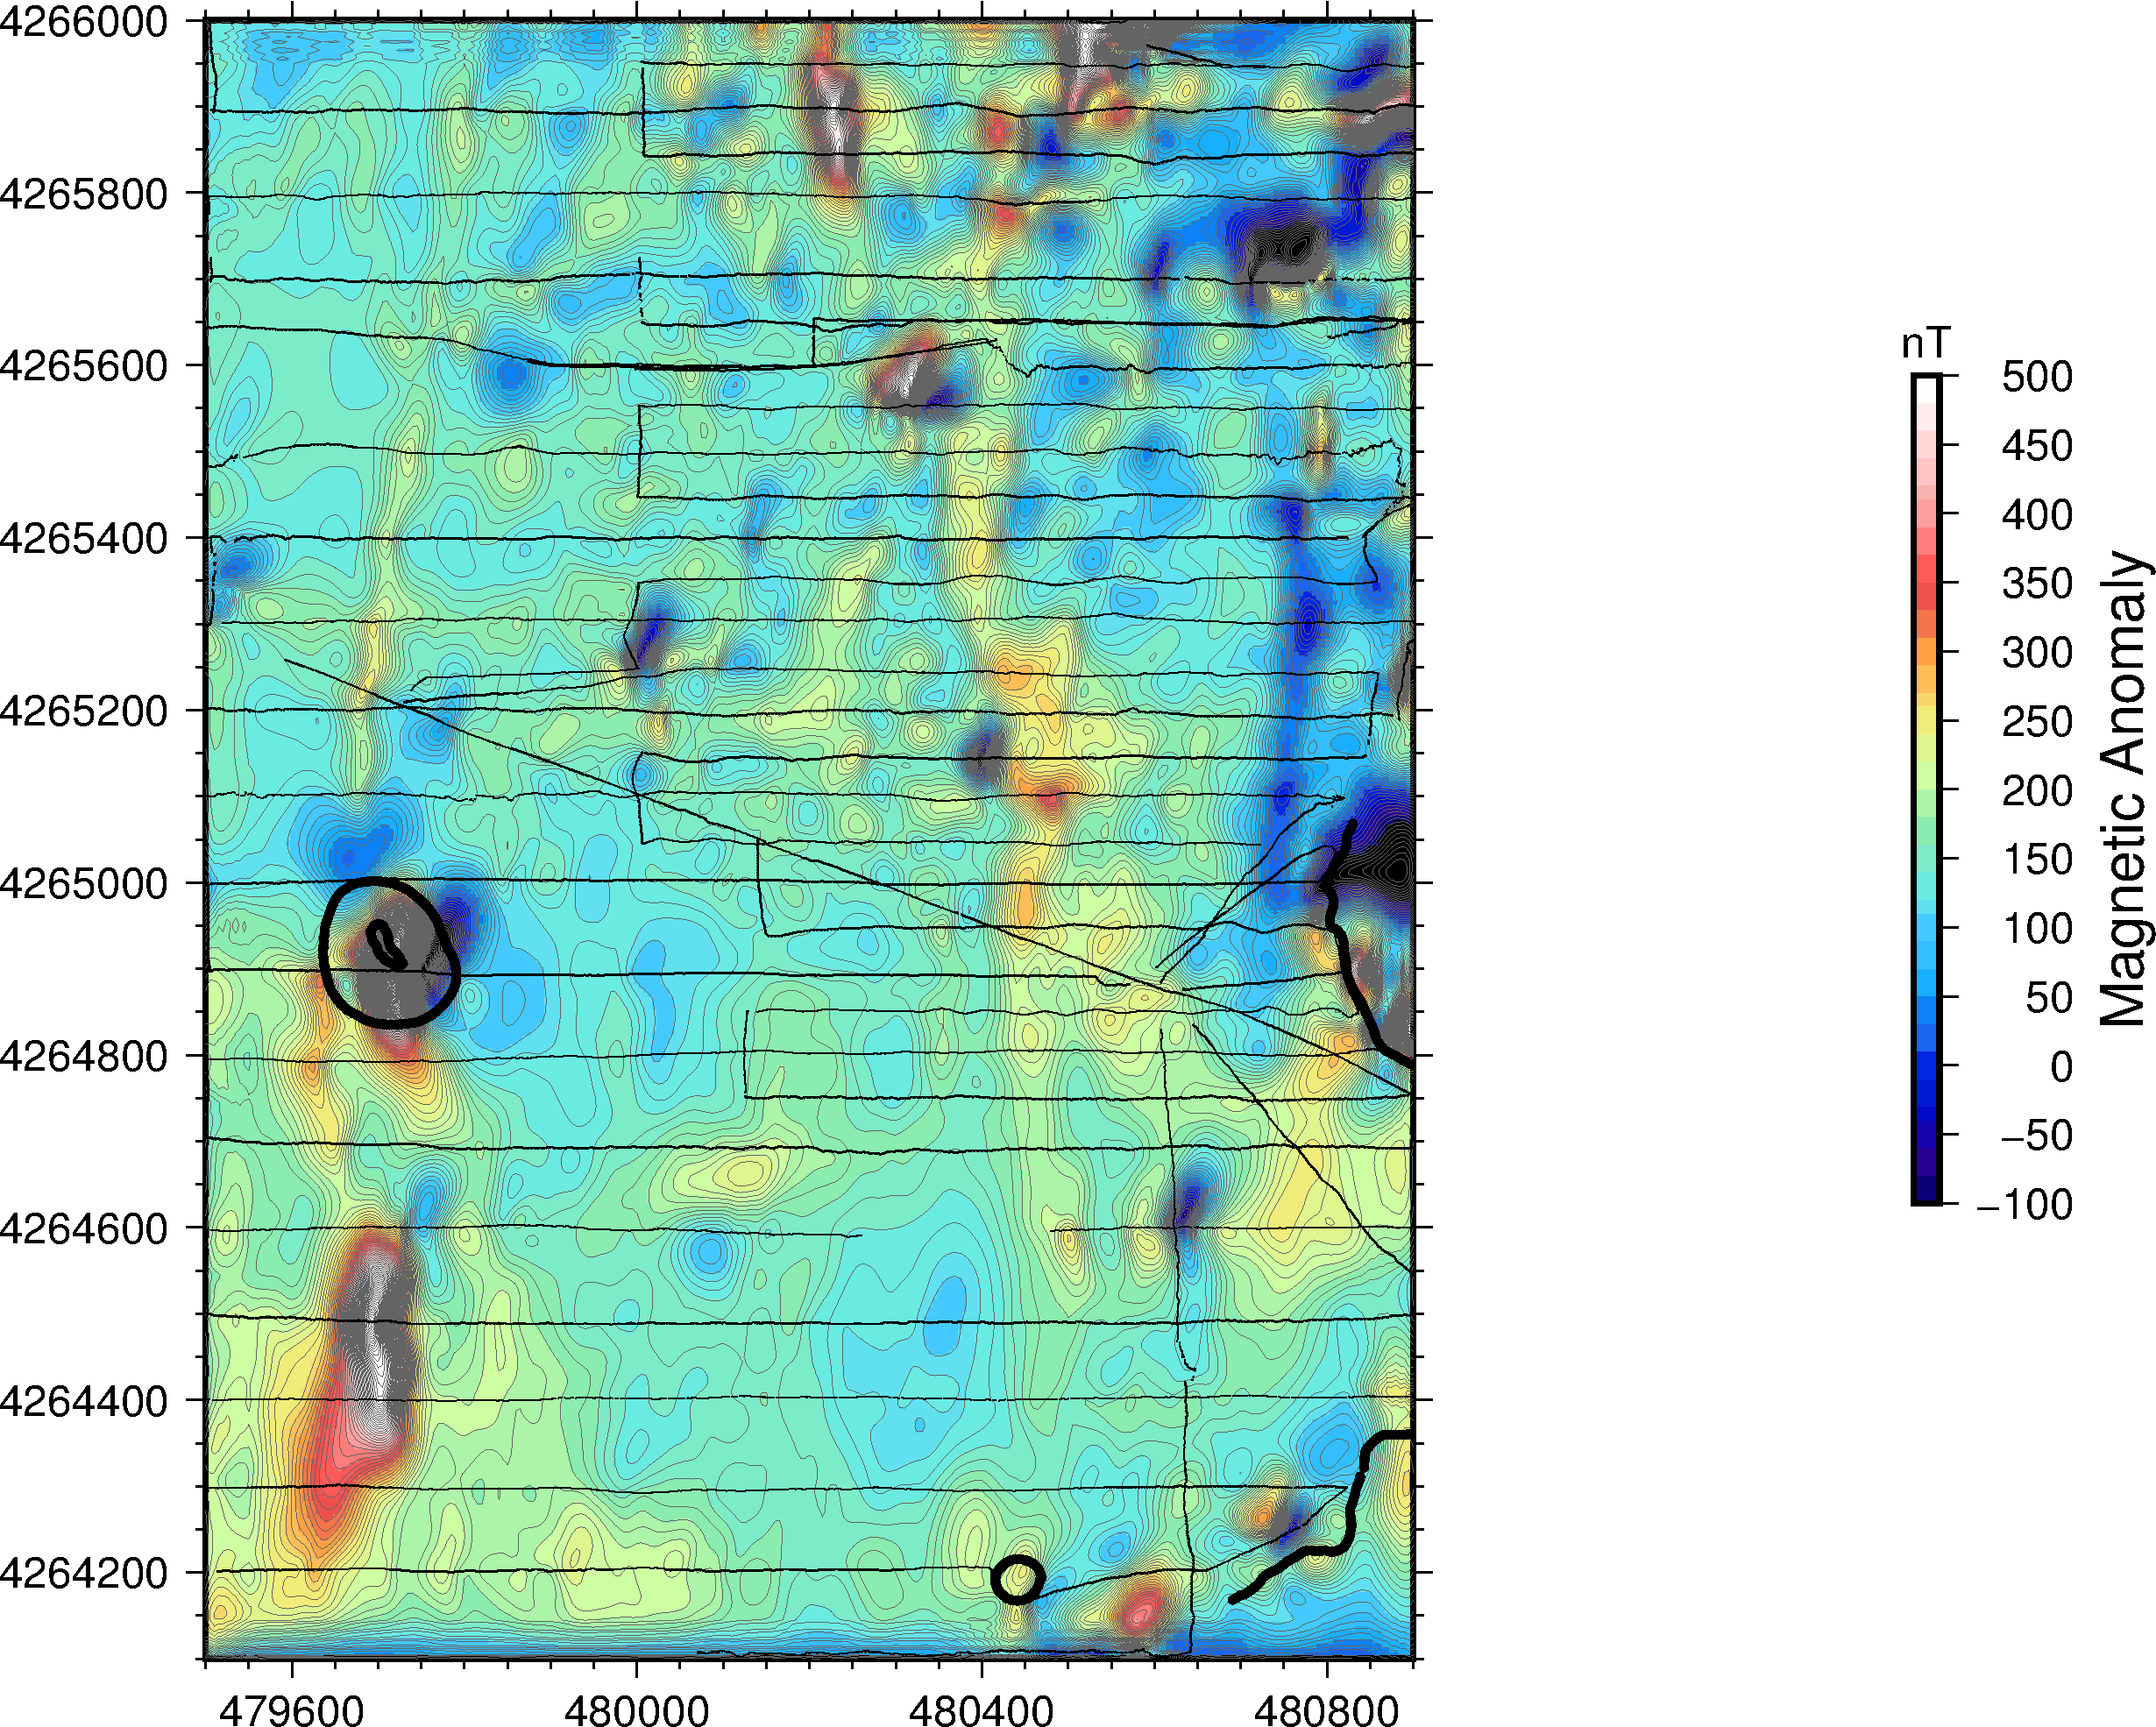
\includegraphics[scale=0.75]{./images/mag_rtp.png}
    \caption{
Output from running the reduction-to-pole procedure described in Step\,6}
    \label{fig:rtp}
\end{figure}


\end{document}

